\documentclass{proposal}
\usepackage{graphicx}
\usepackage[square,numbers]{natbib}
\usepackage{listing}
\usepackage{minted}
\usepackage{chngcntr}
\usepackage[hyphens]{url}
\usepackage{hyperref}

\setminted{frame=lines, linenos, autogobble}

\begin{document}

    \counterwithin{listing}{section}


%%%%%%%%%%%%%%%%%%%%%%%%%%%%%%%%%%%%%%%%%%%%%%%%%%%%%%%%%%%%%%%%%%%%%%%%%%%%%%%%%%%%%%%%%%%%%%%%%%%%%%%%%%%%%%%%%%%%%%%%


    \title{ptr-tidy: Automatic refactoring of raw pointers in C++}
    \author{Artem Usov}
    \date{18 December 2020}
    \maketitle
    \tableofcontents
    \newpage


%%%%%%%%%%%%%%%%%%%%%%%%%%%%%%%%%%%%%%%%%%%%%%%%%%%%%%%%%%%%%%%%%%%%%%%%%%%%%%%%%%%%%%%%%%%%%%%%%%%%%%%%%%%%%%%%%%%%%%%%


    \section{Introduction}\label{sec:intro}

    \subsection{Difficulties with Memory Management}\label{subsec:difficulties-with-memory-management}

    % TODO insert info about what memory management/errors are

    Correct memory management is a difficult problem.

    \emph{How difficult one might ask?}

    In a presentation by Matt Miller, a security engineer at Microsoft~\cite{Miller2019}, it is shown that around 70\% of vulnerabilities that are addressed through a security updates are due to memory safety issues.
    In another presentation at the Linux Security Summit~\cite{Gaynor2020} it is shown that in several other top projects such as Firefox, macOS, Ubuntu and Android all had over half of their CVEs attributed to issues with memory safety.
    This is at industry-leading companies who are renowned for hiring top talent.
    Such memory safety vulnerabilities can be exploited, and due to new regulations such as the GDPR, these issues are more commonly exposed to the general public and punished by regulators.
    Such an example is a fine of £20m fine for a British Airways data breach by the British Information Commissioner's Office~\cite{ICO2020}.

    \subsection{Possible Solutions to Memory Management}\label{subsec:possible-solutions-to-memory-management}

    Memory safety errors occur when languages are used that place the tasks of memory management with the programmer, such as C and C++.
    However simply not using these languages is not an option since their inherent danger makes them highly performant, and therefore the only option for a project such as a web browser.

    \emph{What can be done then to address this issue?}

    Engineers at both Microsoft~\cite{Thomas2019} and Mozilla~\cite{Hostfelt2019} converge on Rust~\cite{Balasubramanian2017} as a possible solution.
    Rust is a systems language that offers the same performance as C and C++~\cite{Lin2016}, however its linear type system and memory ownership model also guarantee memory safety.
    The rewriting of a program in a new language is a colossal undertaking, especially in language that has a reputation for being difficult to learn.
    We therefore propose an alternative partial solution to this problem by using a concept from Rust.


%%%%%%%%%%%%%%%%%%%%%%%%%%%%%%%%%%%%%%%%%%%%%%%%%%%%%%%%%%%%%%%%%%%%%%%%%%%%%%%%%%%%%%%%%%%%%%%%%%%%%%%%%%%%%%%%%%%%%%%%


    \section{Statement of Problem}\label{sec:statement-of-problem}

    \subsection{Using Smart Pointers for Memory Management}\label{subsec:using-smart-pointers-for-memory-management}

    Generally pointers are used to give the program access to a resource that cannot be directly included in the program itself, such as a file or a thread.
    However Stroustrup claims that pointers to objects allocated on the free store is dangerous and a \emph{plain old pointer}, or raw pointer as we will refer to them, should not be used to represent ownership~\cite{Stroustrup2018}.

    \begin{listing}
        \inputminted{c++}{code/manual-leak.cpp}
        \caption{Example of memory leaks using manual management.}
        \label{lst:manual-leak}
    \end{listing}

    In \autoref{lst:manual-leak} we can see that when using a raw pointer, there are two cases in which the programmer will never free the allocated memory.
    Instead we can \emph{smart pointers}~\cite{Dimov2003} and the concept of \emph{RAII (Resource Acquisition Is Initialisation)} to create resource handles which automatically eliminate resource leaks with no added overhead.
    The equivalent code using \emph{unique pointers} can be seen in \autoref{lst:first-example-unique}.
    In the comments, we can see all the locations where \emph{p} exits the scope of the function and where the compiler will insert delete statements, now ensuring that the resource will never get leaked.

    \begin{listing}
        \inputminted{c++}{code/first-example-unique.cpp}
        \caption{Example of using a unique pointer to manage memory.}
        \label{lst:first-example-unique}
    \end{listing}

    There also exists a \emph{shared pointer} for resources which may not have a single unique owner.
    Reference counting is used to ensure that after the last owner loses access to the resource, it will finally be freed.
    Shared pointers are suitable to be used in most situations, except in structures which have cyclic references \autoref{subsec:shared-pointer-cycle-analysis}.

    \subsection{Do Smart Pointer Solve Memory Management?}\label{subsec:do-smart-pointer-solve-memory-management?}

    It would appear then that smart pointers could solve most of our memory management issues, however they were only introduced in the C++11 standard.
    The C++ dialects till then did not have any of these language features, with programs being written predominantly in the C++03 standard.
    There remain many such so called \emph{legacy} programs which have not upgraded to newer standards, and even then, it is up to the programmer to properly utilise smart pointers in their code.

    We therefore propose to create an automatic refactoring tool \emph{(ptr-tidy)}, that statically analyses C++ code and aims to refactor usage of raw pointers into smart pointers.
    It will involve a conservative analysis that first and foremost tries to identify raw pointers that only have a single unique owner at any point in the program.
    If this cannot be guaranteed, then a more conservative refactoring to a shared pointer will be applied.

    Given that the language standards are mostly backwards-compatible~\cite{Winters2020}, we can apply these automatic refactoring without changing the runtime behaviour compared to the original programs.

    % TODO reword section title - or move to proposed approach section

    \subsection{The Research Questions}\label{subsec:the-research-questions}

    \emph{"Can the translation of raw pointers into smart pointers using escape analysis be used to make existing C++ code more modern and extendable?"}

    \emph{"Can the tool identify situations in which unique pointers should be used reliably?"}


%%%%%%%%%%%%%%%%%%%%%%%%%%%%%%%%%%%%%%%%%%%%%%%%%%%%%%%%%%%%%%%%%%%%%%%%%%%%%%%%%%%%%%%%%%%%%%%%%%%%%%%%%%%%%%%%%%%%%%%%


    \section{Background Survey}\label{sec:background-survey}

    In this section we will look into the frameworks and algorithms that we will use to enable us to read and refactor C++ code, and secondly identify the locations where we can apply our refactorings.

    \subsection{Clang and LLVM}\label{subsec:clang-and-llvm}

    C++ as a language is massive, and the first capability our tool will need is to be able to parse C++ code.
    Doing this ourselves would be an undertaking that would likely span longer than the time span of the whole project, therefore it was decided early to use an existing parser.
    The most capable and mature C++ parsers will naturally be the parsers used by the most popular compilers.
    This leaves us therefore with a choice between GCC~\cite{GCC} and Clang~\cite{Clang}.
    The literature~\cite{duffy2014} is fairly clear on the fact that the design of GCC makes it unsuitable for integration with other projects.
    Clang on the other hand allows us access to the Clang abstract syntax tree (AST) and parser internals through consumers and visitors.

    Clang is a front-end to the LLVM framework~\cite{Lattner2004} which transforms C++ code into the LLVM intermediate representation (IR).
    The LLVM IR is a language-independent, static single assignment (SSA) representation of the program and will be the target on which we apply our analysis to identify refactoring opportunities.
    We believe this choice will lead to several benefits in terms of the analysis power and future usage of the project:
    \begin{itemize}
        \item First, the usage of SSA allows us to efficiently generate a definition-usage graph, therefore allowing an efficient analysis of all the usages of a pointer to identify its number of owners.
        \item Secondly, by separating the parsing and analysis, we make our analysis stage reusable by any other LLVM frontends.
    \end{itemize}

    Clang was also found to be a good choice of library in terms of usability since documentation and examples are readily found.
    The AST that it produces is also rich in information and closely resembles the original code, as can be seen in \autoref{lst:code-to-ast-example}.
    Information such as the line and column numbers are included, which makes programmatically rewriting source code extremely easy.

    \begin{listing}
        \inputminted{c++}{code/code-to-ast.cpp}
        \inputminted[fontsize=\footnotesize]{text}{code/code-to-ast.txt}
        \caption{Example of converting C++ code to Clang AST}
        \label{lst:code-to-ast-example}
        % \centerline{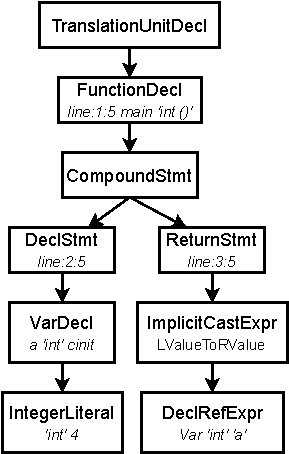
\includegraphics{images/code-to-ast}}
    \end{listing}

    \subsection{Memory Safe Languages}\label{subsec:rust}

    There have been many proposed systems languages such as Rust, Swift \footnote{\url{https://developer.apple.com/swift/}}, D \footnote{\url{https://dlang.org/}}, Nim \footnote{\url{https://nim-lang.org/}} or Ada (SPARK) \footnote{\url{https://adacore.com/}}, however none of these have arguably become mainstream, with Rust and Ada coming closest.

    Swift remains mostly a language for the Apple MacOS and iOS environments for application creation, however it has seen some usage for system programs by companies such as IBM \footnote{\url{https://github.com/ibm-swift}}.
    Ada or its subset language SPARK are used extensively in certain industries to create verifiable programs for critical systems such as in avionics.
    It is perhaps most well-know for being used in the F-22 fighter aircraft~\cite{malas1997f}, however the use of Ada for those systems show its other weakness in productivity time as it was the cause for several delays in the project, and so it largely remains unused in areas which do not call for such meticulous safety.

    Rust has been the most language in attractive widespread adoption as a systems language.
    Its popularity could be quantified by considering that it is being considered for usage in writing Linux kernel modules \footnote{\url{https://lore.kernel.org/lkml/CAKwvOdmuYc8rW_H4aQG4DsJzho=F+djd68fp7mzmBp3-wY--Uw@mail.gmail.com/T}}, which cannot be said for C++.
    Following the advice given by many that most systems programs should be written in Rust from now on, we see a potential future usage of our work in the creation of a C++ to Rust transpiler.

    Whilst the automatic refactoring of raw pointers into smart pointers solves some memory issues, the language still offers other ways to invalidate memory safety.
    Equivalent idiomatic Rust would be able to find some of these other errors at compile time.
    A C++ to Rust transpiler would be a much larger undertaking, however we can envision how our project could be helpful.
    Rust affine types~\cite{Balasubramanian2017} are semantically equivalent to C++ unique pointers, in that all values have a single unique owner at any point.
    Therefore our work can identify which pointers are unique and which are not, and those that are not cannot be transpiled into safe Rust, instead requiring to use unsafe blocks to represent such values.


%%%%%%%%%%%%%%%%%%%%%%%%%%%%%%%%%%%%%%%%%%%%%%%%%%%%%%%%%%%%%%%%%%%%%%%%%%%%%%%%%%%%%%%%%%%%%%%%%%%%%%%%%%%%%%%%%%%%%%%%


    \section{Proposed Approach}\label{sec:proposed-approach}

    State how you propose to solve the software development problem.
    Show that your proposed approach is feasible, but identify any risks.

    \subsection{Shared Pointer Cycle Analysis}\label{subsec:shared-pointer-cycle-analysis}

%%%%%%%%%%%%%%%%%%%%%%%%%%%%%%%%%%%%%%%%%%%%%%%%%%%%%%%%%%%%%%%%%%%%%%%%%%%%%%%%%%%%%%%%%%%%%%%%%%%%%%%%%%%%%%%%%%%%%%%%


    \section{Work Plan}\label{sec:work-plan}

    Show how you plan to organize your work, identifying intermediate deliverables and dates.


%%%%%%%%%%%%%%%%%%%%%%%%%%%%%%%%%%%%%%%%%%%%%%%%%%%%%%%%%%%%%%%%%%%%%%%%%%%%%%%%%%%%%%%%%%%%%%%%%%%%%%%%%%%%%%%%%%%%%%%%


    \bibliographystyle{plainnat}
    \bibliography{proposal}
\end{document}
